\chapter{Performance and Fault Tolerance}
\label{ch:performance}

Tendermint is designed as a Byzantine fault tolerant state-machine replication algorithm.
It gaurantees safety so long as less than a third of validators are Byzantine, 
and gaurantees liveness similarly, so long as network messages are eventually delivered,
with weak assumptions about network synchrony for gossipping proposals.
In this section, we evaluate Tendermint's fault tolerance empirically by injecting 
crash faults, Byzantine faults, and arbitrary network delays.
The goal is to show that the implementation of Tendermint consensus does not compromise safety in the event of such failures,
that it suffers minimum performance impact, and that it is quick to recover.

Performance of the Tendermint algorithm can be evaluated in a few key ways.
The most obvious measures are the block commit time, which is a measure of finalization latency, 
and transaction throughput, which measures the network's capacity.
We collect measurements for each on networks with validators distribtued over the globe, 
where the number of validators ranges, in multiples of 2, from 2 to 64.

\section{Overview}

The experiments in this chapter can be reproduced using the repository at https://github.com/tendermint/network\_testing.
All experiments take place in docker containers running on Amazon EC2 instances of type t2.medium.
Instances are distribtued across seven datacenters, spanning five continents (Figure \ref{fig:experiments_overview}).
A second docker container, responsible for generating transactions, is run on each instance.
Transactions are 250 bytes in size (a reasonable size for including a few 32/64 byte hashes and signatures),
where the leading bytes are big endian encoded integers representing transaction number and validator index for that instance,
the trailing 16 bytes are randomly draw from the operating system, and the intermediate bytes are just zeroes.

A network monitoring tool is used to maintain active websocket connections to each validator's tendermint rpc server,
and uses its local time when it receives a new committed block for the first time as the official commit time for that block.
Experiments were first run without the monitor by copying all data from validators for analysis and using the local time
of the 2/3th validator committing a block as the commit time. 
Using the monitor is much faster, ammenable to online monitoring, and was found to not impact the results 
so long as only block header information (and not the whole block) was passed over the websockets.

Docker containers on remote machines are easily managed using the docker-machine tool, 
and the network\_testing repository provides some tools which take advantage of go's concurrency features
to perform actions on docker containers on many remote machines at once.

Each validator connects directly to each other to avoid confounding effects of network topology.

For experiments involving crash faults or byzantine behaviour, the number of faulty nodes is given by $N_{fault} = (N-1)/3$.

\section{Throughput and Latency}

This section describes experiments which measure the raw performance of tendermint in non-adversarial conditions,
where all nodes are online and synced and no accomodations are made for asynchrony.
That is, an artifically high TimeoutPropose is used (10 seconds), and all other timeout parameters are set to 1 millisecond.
Additionally, all mempool activity is disabled (no gossip transactions or rechecking them after commits),
and an in-process nil application is used to bypass TMSP.
This serves as a control scenario for evaluating the performance drop in the face of faults and/or asynchrony.

Experiments are run on validator set sizes doubling in size from two to 64, and on block sizes doubling from 128 to 32768.
Transactions are preloaded on each validator. Each experiment is run for 16 blocks. 

As can be seen in Figure \ref{fig:exp:throughput_latency}, 
tendermint easily handles thousands of transactions per second with around one second block latency,
though there appears to be a capacity limit at around ten thousand transactions per second.
A block of 16384 transactions is about 4 MB in size, and analysis of network bandwidth shows each connection
easily reaching upwards of 20MB/s, though analysis of the logs shows that at high block sizes, 
validators can spend upwards of two seconds waiting for block parts.
Transaction throughput as a function of blocksize is shown in \ref{fig:exp:throughput_blocksize}
Thus it is likely that a more efficient block-part broadcast algorithm may alleviate this bottleneck.
Additionally, experiments in single data centers, as shown in Figure \ref{fig:exp:single},
demonstrate that much higher throughputs are possible. We leave further investigations of this capacity limit to future work.


\begin{figure}[]
	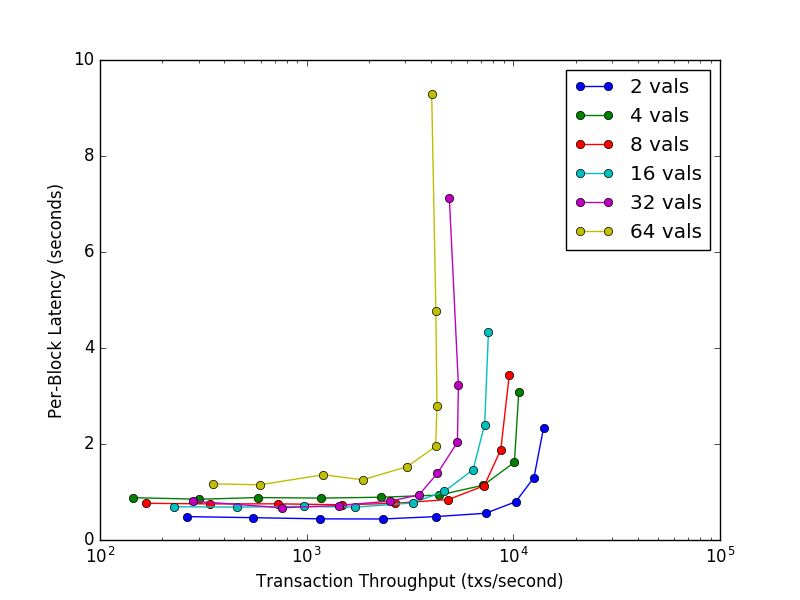
\includegraphics[width=\linewidth,height=\textheight,keepaspectratio]{figures/throughput/latency-throughput.png}
    	\centering
	\label{fig:exp:throughput_latency}
	\caption[Latency-throughput in non-faulty network]{Latency-throughput tradeoff on nodes distributed around the globe}
\end{figure}
\begin{figure}[]
	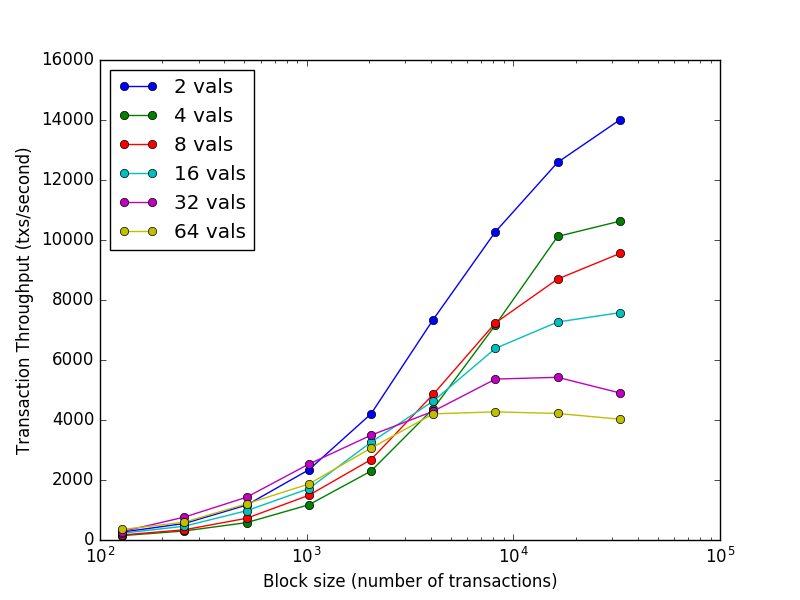
\includegraphics[width=\linewidth,height=\textheight,keepaspectratio]{figures/throughput/throughput-blocksize.png}
    	\centering
	\label{fig:exp:throughput_blocksize}
	\caption[Throughput-blocksize in non-faulty network]{Larger blocks incur diminishing returns in transaction throughput, with an ultimate capacity at around 10,000 txs/s}
\end{figure}
\begin{figure}[]
	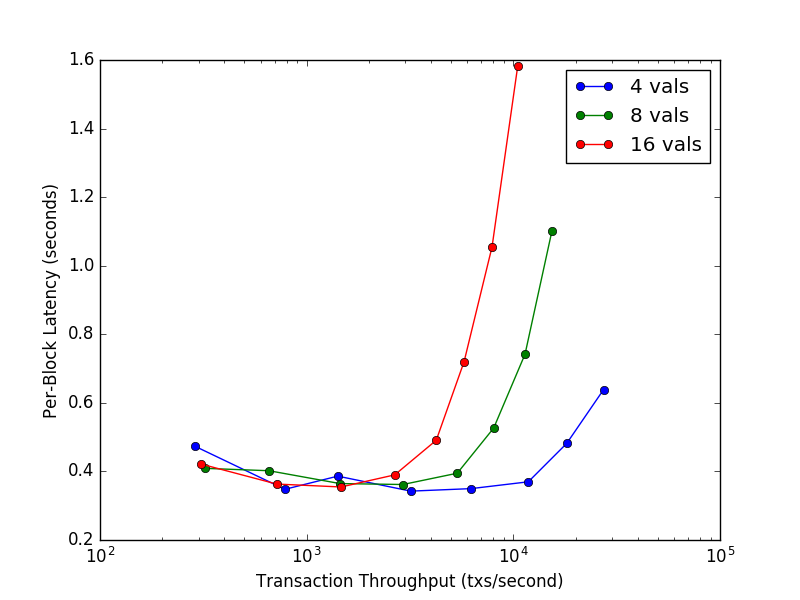
\includegraphics[width=\linewidth,height=\textheight,keepaspectratio]{figures/single_datacenter/latency-throughput.png}
    	\centering
	\label{fig:exp:single}
	\caption[Latency-throughput in non-faulty network, single data center]{Latency-throughput tradeoff in a single datacenter shows tendermint is capable of tens of thousands of transactions per second}
\end{figure}

\section{Crash Failures and Asynchrony}

To evaluate the performance due to crash failures, every three seconds $N_{fault}$ validators are randomly selected,
stopped, and restarted three seconds later.
Experiments are run for validator set sizes doubling from 2 to 64, for varying values of TimeoutPropose.
In each experiment, the block size is 2048.

The results in Figure \ref{fig:exp:crash_failure} demonstrate that performance under this crash failure scenario drops by about 
$50\%$, and that larger TimeoutPropose values help mediate latencies. While the average latency increases towards three seconds,
the median is closer to one second, and latencies may run as high as ten seconds.

Crash failures are closely related to asynchrony, as it can be difficult to distinguish between a crashed node
and delayed messages. A variety of heuristics exist, such as using pings, 
but in each case they require an assumption of some synchrony. 
To evaluate performance in the face of network asynchrony, twenty percent of all messages are delayed an amount of time chosen uniformly 
from one to ten seconds.

\begin{figure}[]
	Crash-fault latency statistics	
	4 Validators

\begin{center}
	\begin{tabular}{| l | l | l | l | l | l | }
		\hline
		TimeoutPropose & Min & Max & Mean & Median & $95^{th} \ \%-ile$ \\ \hline
		500 & 434 & 15318 & 2179 & 1102 & 5575 \\ \hline
		1000 & 516 & 18149 & 2180 & 1046 & 5677 \\ \hline
		2000 & 473 & 15067 & 2044 & 1049 & 5479 \\ \hline
		3000 & 428 & 9964 & 2005 & 1096 & 5502 \\ \hline
	\end{tabular}
\end{center}

8 Validators

\begin{center}
	\begin{tabular}{| l | l | l | l | l | l | }
		\hline
		TimeoutPropose & Min & Max & Mean & Median & $95^{th} \ \%-ile$ \\ \hline
		500 & 618 & 126481 & 2679 & 990 & 5589 \\ \hline
		1000 & 570 & 9832 & 1763 & 962 & 5835 \\ \hline
		2000 & 594 & 8869 & 1658 & 968 & 5481 \\ \hline
		3000 & 535 & 10101 & 1633 & 959 & 5485 \\ \hline
	\end{tabular}
\end{center}

16 Validators

\begin{center}
	\begin{tabular}{| l | l | l | l | l | l | }
		\hline
		TimeoutPropose & Min & Max & Mean & Median & $95^{th} \ \%-ile$ \\ \hline
		500 & 782 & 21354 & 1977 & 1001 & 5930 \\ \hline
		1000 & 758 & 12659 & 1761 & 981 & 5642 \\ \hline
		2000 & 751 & 21285 & 2041 & 1005 & 6872 \\ \hline
		3000 & 719 & 72406 & 2395 & 991 & 5987 \\ \hline
	\end{tabular}
\end{center}

32 Validators

\begin{center}
	\begin{tabular}{| l | l | l | l | l | l | }
		\hline
		TimeoutPropose & Min & Max & Mean & Median & $95^{th} \ \%-ile$ \\ \hline
		500 & 760 & 24692 & 2591 & 1087 & 14025 \\ \hline
		1000 & 755 & 19696 & 2328 & 1119 & 9321 \\ \hline
		2000 & 852 & 21044 & 2178 & 1141 & 6514 \\ \hline
		3000 & 763 & 25587 & 2289 & 1119 & 6707 \\ \hline
	\end{tabular}
\end{center}


	\label{fig:exp:crash_failure}
	\caption[Latency statistics under crash faults]{Every three seconds, a random $(N-1)/3$ validators were crashed, and restarted three seconds later. This crash-restart procedure continued for 200 blocks. Each table reports the minimum, maximum, average, median, and $95^{th}$ percentile of the block latencies, for varying values of the TimeoutPropose parameter.}
\end{figure}


\section{Byzantine Failures}

Since its infeasible to capture every instance of arbitrary behaviour,
a few implementations are provided which cover some important cases, namely:
network fuzzing, double signing proposals or votes, and violating locking rules.

\subsection{Network fuzzing}

To simulate network fuzzing, $N_{fault}$ validators randomly corrupt 25\% of the bytes in 10\% of the messages they send.

\subsection{Double signing}

To simulate a more determined byzantine adversary, the consensus state machine is augmented to allow explicit byzantine behaviour.
In particular, for this experiment, a byzantine validator makes the following changes.

\begin{itemize}
\item{Conflicting proposals: during its time to propose, a byzantine validator signs two conflicting proposals and broadcasts each, along with a prevote and precommit, to separate halves of its connected peers.} 
\item{No nil votes: a byzantine validator signs no nil-votes, no matter what}
\item{Sign every proposal: a byzantine validator submits a prevote and a precommit for every proposal it sees, as soon as it sees it}
\end{itemize}

Taken together, these behaviours explicilty violate the double signing and locking rules. 

\begin{figure}[]
	Byzantine-fault latency statistics	
	4 Validators

\begin{center}
	\begin{tabular}{| l | l | l | l | l | l | }
		\hline
		TimeoutPropose & Min & Max & Mean & Median & $95^{th} \ \%-ile$ \\ \hline
		1000 & 868 & 3888 & 1450 & 1086 & 3320 \\ \hline
		2000 & 929 & 4375 & 1786 & 1272 & 4166 \\ \hline
		3000 & 881 & 4363 & 1224 & 1099 & 1680 \\ \hline
		4000 & 824 & 8256 & 1693 & 1272 & 2607 \\ \hline
	\end{tabular}
\end{center}

8 Validators

\begin{center}
	\begin{tabular}{| l | l | l | l | l | l | }
		\hline
		TimeoutPropose & Min & Max & Mean & Median & $95^{th} \ \%-ile$ \\ \hline
		1000 & 771 & 3445 & 1472 & 916 & 3288 \\ \hline
		2000 & 731 & 3661 & 1426 & 902 & 3339 \\ \hline
		3000 & 835 & 6402 & 1912 & 962 & 6155 \\ \hline
		4000 & 811 & 4462 & 1512 & 964 & 3592 \\ \hline
	\end{tabular}
\end{center}

16 Validators

\begin{center}
	\begin{tabular}{| l | l | l | l | l | l | }
		\hline
		TimeoutPropose & Min & Max & Mean & Median & $95^{th} \ \%-ile$ \\ \hline
		1000 & 877 & 15930 & 2086 & 1024 & 5844 \\ \hline
		2000 & 808 & 5737 & 1580 & 1027 & 4155 \\ \hline
		3000 & 919 & 10533 & 1801 & 1110 & 4174 \\ \hline
		4000 & 915 & 5589 & 1745 & 1095 & 4181 \\ \hline
	\end{tabular}
\end{center}

32 Validators

\begin{center}
	\begin{tabular}{| l | l | l | l | l | l | }
		\hline
		TimeoutPropose & Min & Max & Mean & Median & $95^{th} \ \%-ile$ \\ \hline
		1000 & 1594 & 11730 & 2680 & 1854 & 5016 \\ \hline
		2000 & 1496 & 17801 & 3430 & 1874 & 11730 \\ \hline
		3000 & 1504 & 15963 & 3280 & 1736 & 9569 \\ \hline
		4000 & 1490 & 24836 & 3940 & 1773 & 12866 \\ \hline
	\end{tabular}
\end{center}


	\label{fig:exp:byz_failure}
	\caption[Latency statistics under byzantine faults]{$(N-1)/3$ validators were set to be byzantine.
Byzantine validators propose conflicting blocks and vote on any proposal as soon as they see it.
Each table reports the minimum, maximum, average, median, and $95^{th}$ percentile of the block latencies, for varying values of the TimeoutPropose parameter.}
\end{figure}


\section{A real application: ErisDB}

The experiments presented so far have been artificial to the extent that transactions incur no processing logic.
This was done deliberately to benchmark the core consensus engine. 
To get a handle on a real application, we present throughput and latency results for ErisDB, 
a blockchain application developed primarily by the author at Eris Industries, in collaboration with Jae Kwon.
ErisDB provides a rich set of features, including a native currency, the Ethereum Virtual Machine (EVM).
a native name registry, and a rich permissioning system.
Transactions must be digitally signed using ED25519 signatures to be valid, and all state queries and updates are done on a merkle IAVL tree.

For this experiment, a simple contract with two methods, get and set, is deployed to the virtual machine.
The contract is written in solidity, a high-level, javascript-like language developed by Ethereum which compiles down to EVM byte code.
The application state is preloaded with 1000 accounts, and transactions are signed by private keys drawn uniformly from those accounts.
Keys and values for the get and set methods are fixed at 32-bytes each, to reflect the native architecture of the EVM \ref{ethereum_yellow_paper}.
Transactions are generated for a read/write load of 10/90 (i.e. 90\% of transaction call the set method).

\section{Related Work}
